\begin{figure}[!htbp]\centering
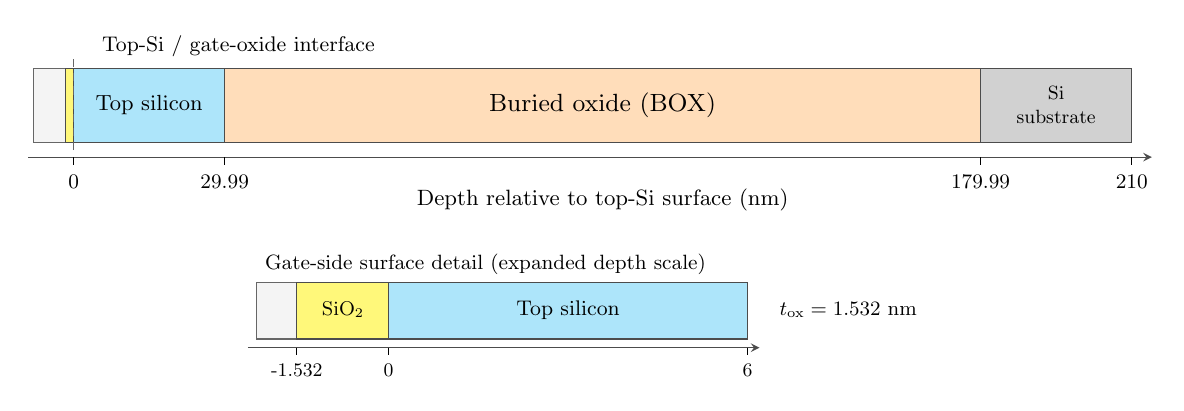
\begin{tikzpicture}[x=.064cm,y=1cm,font=\small]
  % SProcess depth referenced to oxide/Si interface X=-0.17998572 um.
  \draw[fill=gray!9,draw=black!60] (-8,.5) rectangle (-1.53231,1.44);
  \draw[fill=yellow!52,draw=black!70] (-1.53231,.5) rectangle (0,1.44);
  \draw[fill=cyan!32,draw=black!70] (0,.5) rectangle (29.98571,1.44);
  \draw[fill=orange!27,draw=black!70] (29.98571,.5) rectangle (179.98572,1.44);
  \draw[fill=gray!36,draw=black!70] (179.98572,.5) rectangle (210,1.44);
  \node[scale=.88] at (14.99,.97) {Top silicon};
  \node at (104.98,.97) {Buried oxide (BOX)};
  \node[align=center,scale=.77] at (194.99,.97) {Si\\substrate};
  \draw[densely dashed,black!60] (0,.4)--(0,1.61);
  \node[anchor=west,scale=.85] at (4,1.72) {Top-Si / gate-oxide interface};
  \draw[-stealth,black!70] (-9,.31)--(214,.31);
  \foreach \xx/\lab in {0/0,29.98571/29.99,179.98572/179.99,210/210}{
      \draw (\xx,.31)--(\xx,.21);
      \node[anchor=north,scale=.83] at (\xx,.18) {\lab};
  }
  \node[scale=.89] at (105,-.24) {Depth relative to top-Si surface (nm)};
  % Surface oxide measured at 1.53231 nm: explicit enlarged inset.
  \begin{scope}[xshift=4cm,yshift=-1.65cm,x=.76cm,y=1cm,font=\small]
    \node[anchor=west,scale=.83] at (-2.2,.60) {Gate-side surface detail (expanded depth scale)};
    \draw[fill=gray!9,draw=black!60] (-2.2,-.35) rectangle (-1.53231,.37);
    \draw[fill=yellow!52,draw=black!70] (-1.53231,-.35) rectangle (0,.37);
    \draw[fill=cyan!32,draw=black!70] (0,-.35) rectangle (6,.37);
    \node[scale=.80] at (-.76,.02) {SiO$_2$};
    \node[scale=.85] at (3,.02) {Top silicon};
    \draw[-stealth,black!70] (-2.35,-.46)--(6.2,-.46);
    \foreach \xx/\lab in {-1.53231/{-1.532},0/0,6/6}{
      \draw (\xx,-.46)--(\xx,-.55);
      \node[anchor=north,scale=.77] at (\xx,-.57) {\lab};
    }
    \node[anchor=west,scale=.82] at (6.4,.02) {$t_{\rm ox}=1.532$ nm};
  \end{scope}
\end{tikzpicture}
\caption{Original one-dimensional gate-oxidation SProcess stage
\texttt{soi\_01\_gateoxide\_fps.tdr}, reconstructed from the
exported region-interface coordinates. A 1.532-nm surface oxide
forms above the top silicon ($X=-0.18151803$ to
$-0.17998572\,\mu$m), while the remaining silicon thickness
is 29.986 nm and the BOX is 150.000 nm. The inset uses a
separate, explicitly expanded scale to resolve the oxide.
Both diagrams are plotted from authentic TDR boundaries,
not simulated 2D screenshots.}
\label{fig:gate_oxide_material_profile}
\end{figure}
